\documentclass[a4]{article}

\usepackage[left=2cm,right=2cm,top=2cm,bottom=2cm]{geometry} 

\usepackage[utf8]{inputenc}   % otra alternativa para los caracteres acentuados y la "ñ"
\usepackage[           spanish % para poder usar el español
                      ,es-tabla % para los captions de las tablas
                       ]{babel}   
\decimalpoint %para usar el punto decimal en vez de coma para los números con decimales

%\usepackage{beton}
%\usepackage[T1]{fontenc}

\usepackage{parskip}
\usepackage{xcolor}

\usepackage{caption}

\usepackage{enumerate} % paquete para poder personalizar fácilmente la apariencia de las listas enumerativas

\usepackage{graphicx} % figuras
\usepackage{subfigure} % subfiguras

\usepackage{amsfonts}
\usepackage{amsmath}
\usepackage{listings}
\lstset{language=Python}          % Set your language (you can change the language for each code-block optionally)

\definecolor{gris}{RGB}{220,220,220}
	
\usepackage{float} % para controlar la situación de los entornos flotantes

\restylefloat{figure}
\restylefloat{table} 
\setlength{\parindent}{0mm}


\usepackage[bookmarks=true,
            bookmarksnumbered=false, % true means bookmarks in 
                                     % left window are numbered
            bookmarksopen=false,     % true means only level 1
                                     % are displayed.
            colorlinks=true,
            allcolors=blue,
            urlcolor=cyan]{hyperref}
\definecolor{webblue}{rgb}{0, 0, 0.5}  % less intense blue


\title{\Huge Inteligencia de Negocio. Práctica 2:\\
Visualización y Segmentación \vspace{5mm}}

\author{\LARGE Patricia Córdoba Hidalgo \vspace{2mm}\\
  \Large patriciacorhid@correo.ugr.es \vspace{2mm}\\
  \Large Grupo 2 (Viernes) \vspace{5mm}}

\date{\today}

\begin{document}

\maketitle

\newpage
\tableofcontents
\newpage

\section{Visualización}

\subsection{Visualización de medidas}

En la práctica 1 se mostraron los datos de cada una de las medidas en tablas, mostrando el valor numérico de éstas. Otra forma de mostrar estos datos es mediante gráficas. En esta práctica, se mostrarán en diagramas de barras los valores de las medidas más utilizadas para la toma de decisiones en la práctica anterior.

Veamos primero los resultados de los diferentes preprocesados de datos:

\begin{center}
  \textbf{Procesado 1}
\end{center}

\begin{figure}[H]
  \centering
  \subfigure[Accuracy]{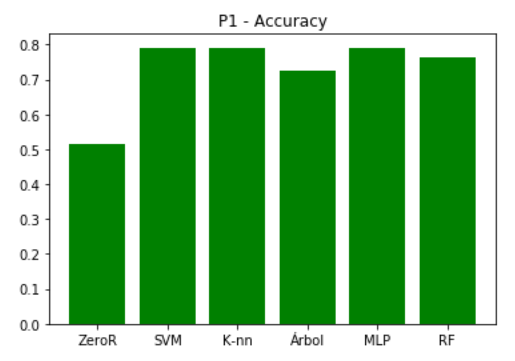
\includegraphics[width=43mm]{imagenes/p1_acc}}
  \subfigure[F1-Score]{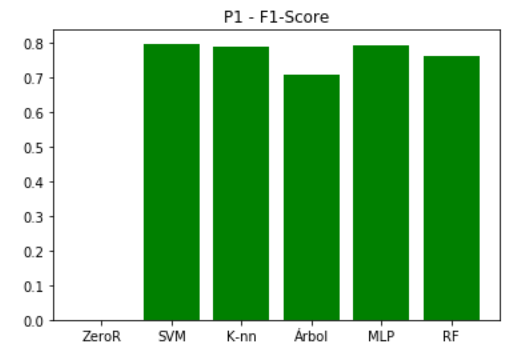
\includegraphics[width=43mm]{imagenes/p1_f1}}
  \subfigure[TPR]{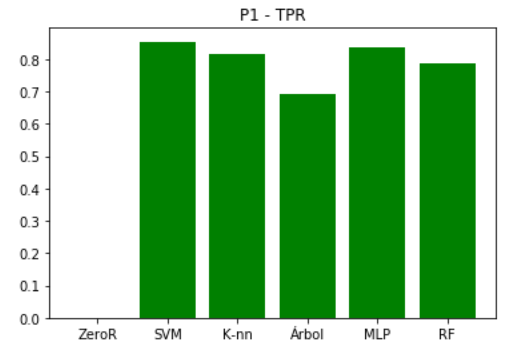
\includegraphics[width=43mm]{imagenes/p1_tpr}}
  \subfigure[FNR]{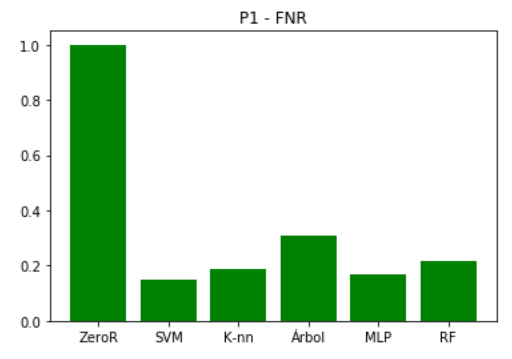
\includegraphics[width=43mm]{imagenes/p1_fnr}}
\end{figure}

\vspace{-5mm}

\begin{center}
  \textbf{Procesado 2}
\end{center}

\begin{figure}[H]
  \centering
  \subfigure[Accuracy]{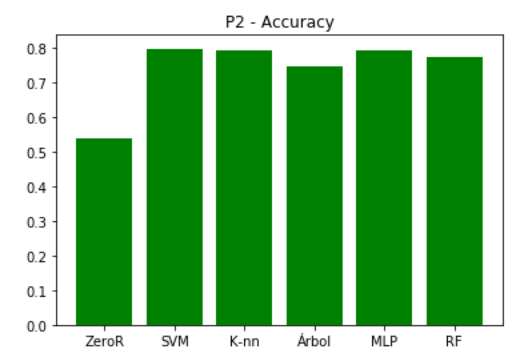
\includegraphics[width=43mm]{imagenes/p2_acc}}
  \subfigure[F1-Score]{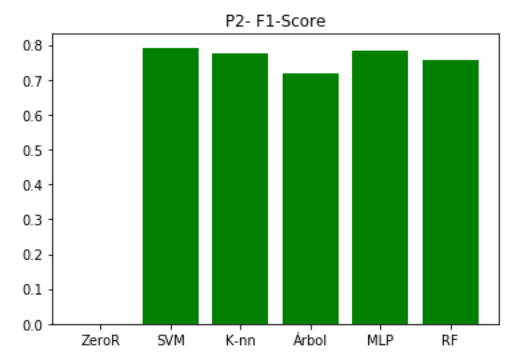
\includegraphics[width=43mm]{imagenes/p2_f1}}
  \subfigure[TPR]{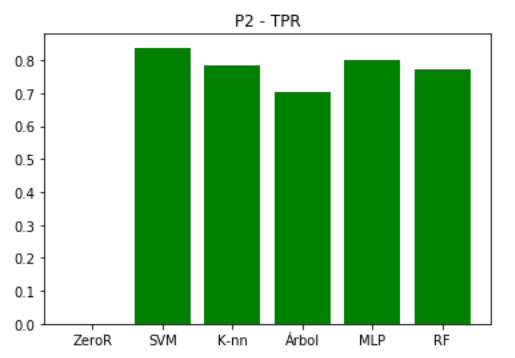
\includegraphics[width=43mm]{imagenes/p2_tpr}}
  \subfigure[FNR]{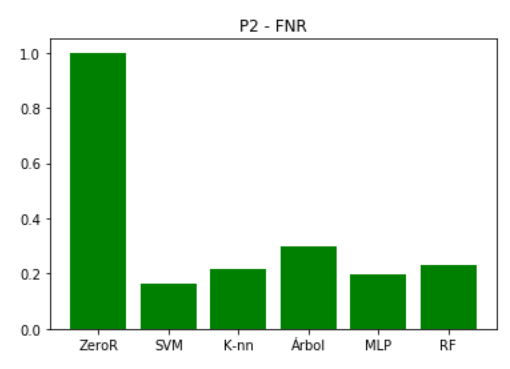
\includegraphics[width=43mm]{imagenes/p2_fnr}}
\end{figure}

\vspace{-5mm}

\begin{center}
  \textbf{Procesado 3}
\end{center}

\begin{figure}[H]
  \centering
  \subfigure[Accuracy]{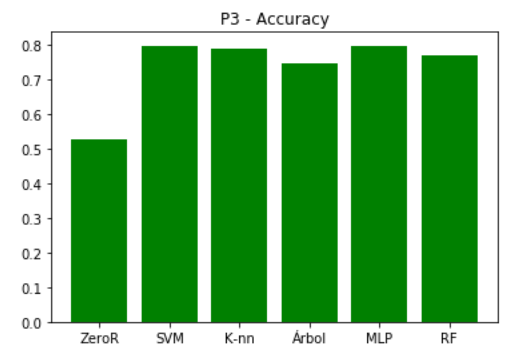
\includegraphics[width=43mm]{imagenes/p3_acc}}
  \subfigure[F1-Score]{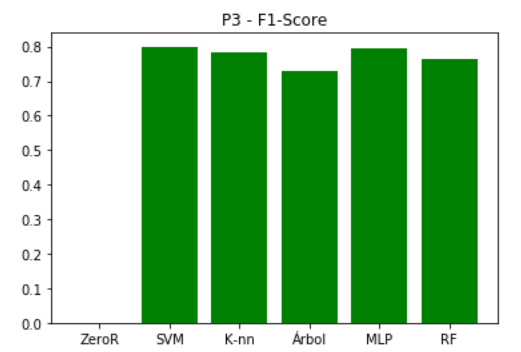
\includegraphics[width=43mm]{imagenes/p3_f1}}
  \subfigure[TPR]{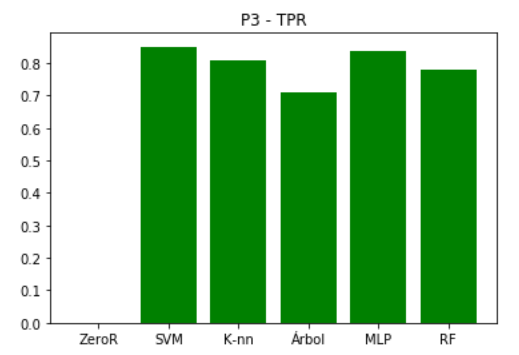
\includegraphics[width=43mm]{imagenes/p3_tpr}}
  \subfigure[FNR]{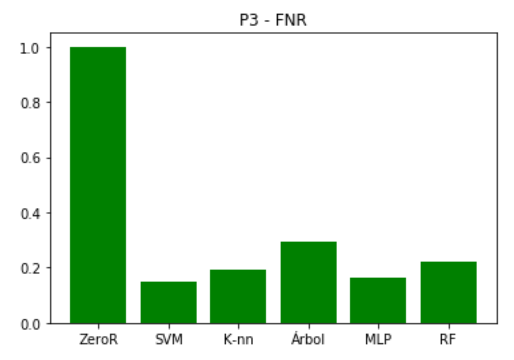
\includegraphics[width=43mm]{imagenes/p3_fnr}}
\end{figure}

\vspace{-5mm}

El código de cada gráfica es:

\begin{lstlisting}
fig, ax = plt.subplots()
ax.bar(["ZeroR", "SVM", "K-nn", "Arbol", "MLP", "RF"], pX_metrica, color='green')
ax.set_title("PX-metrica")
\end{lstlisting}

Donde ``X'' es denota el preprocesado que se ha aplicado, $1, 2$ o $3$, y `` metrica'' la métrica que se mide, pudiendo ser \texttt{accuracy}, \texttt{F1-Score}, \texttt{TPR} o \texttt{FNR}. El vector pX-metrica es un vector donde se guardan los valores de la métrica ``metrica'' con el preprocesado ``X'' de todos los modelos considerados.

Podemos observar que los tres preprocesados obtienen resultados muy similares, como ya comentamos en la práctica anterior. A primera vista, la estructura de los diagramas parece la misma, es decir, al ordenar los diferentes modelos según el valor de la métrica correspondiente con cada procesamiento, este orden es muy parecido en todos ellos, no atreviéndome a decir el mismo por haber barras de alturas semejantes. Es por esto que decantarse por un procesamiento con estos gráficos resulta complicado.

En los tres preprocesamientos el modelo con menor \texttt{accuracy} es el ZeroR, seguido del árbol de decisión. El SVM, K-nn y MLP son los modelos con mayor \texttt{accuracy} en los tres casos. En el resto de métricas se obserba que el SVM y el MLP tienen un mejor desempeño que el K-nn, siendo estos dos modelos los que mejores resultados obtienen. El árbol de decisión y el ZeroR son los modelos que peor desempeño tienen. El Random Forest y el árbol de decisión no obtienen tan buenos resultados como los otros modelos inicialmente pero, como vimos en la práctica 1, aplicando la poda coste-complejidad obteniamos una gran mejora de su desempeño, ya que con esta poda se conseguía reducir el sobreajuste del modelo.

Para elegir que procesamiento utilizabamos en la práctica 1, nos decantamos por el procesamiento que en más modelos tuviese mayor \texttt{F1-Score}. En las siguientes gráficas mostramos el valor de esta métrica en los diferentes modelos para cada procesamiento: 

\begin{figure}[H]
  \centering
  \subfigure[ZeroR]{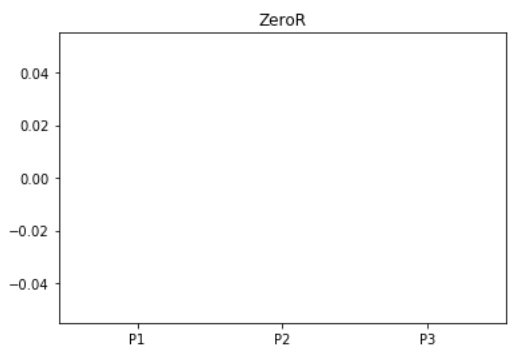
\includegraphics[width=57mm]{imagenes/zeror}}
  \subfigure[SVM]{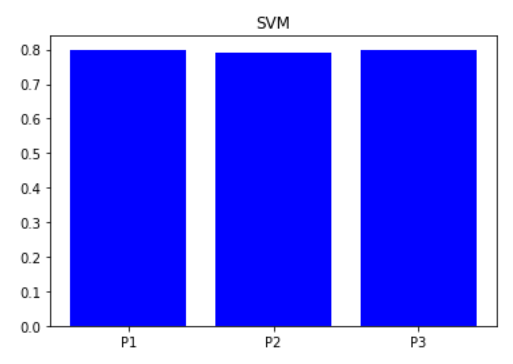
\includegraphics[width=57mm]{imagenes/svm}}
  \subfigure[k-nn]{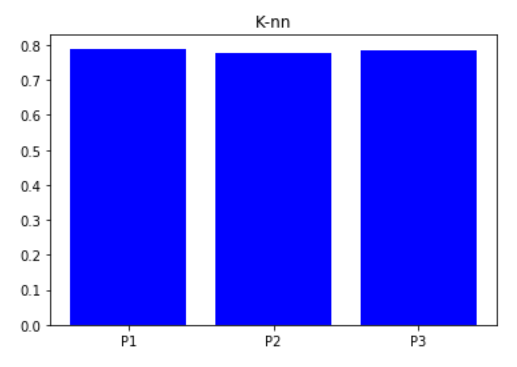
\includegraphics[width=57mm]{imagenes/knn}}
\end{figure}

\begin{figure}[H]
  \centering
  \subfigure[Árbol de decisión]{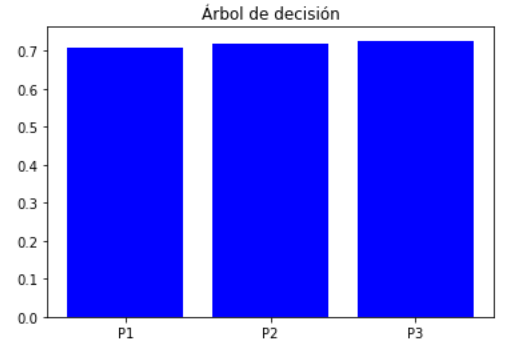
\includegraphics[width=58mm]{imagenes/arbol}}
  \subfigure[MLP]{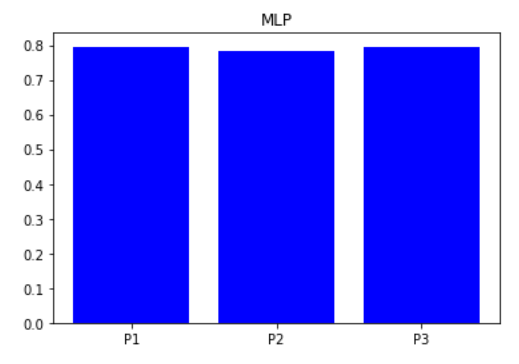
\includegraphics[width=55mm]{imagenes/mlp}}
  \subfigure[Random Forest]{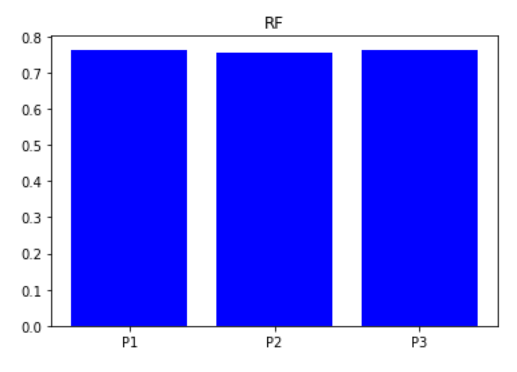
\includegraphics[width=60mm]{imagenes/rf}}
\end{figure}

Como ya hemos visto antes, no hay gran diferencia entre unos y otros. 

\subsection{Curva ROC}

\begin{figure}[H]
  \centering
  \subfigure[Curva ROC]{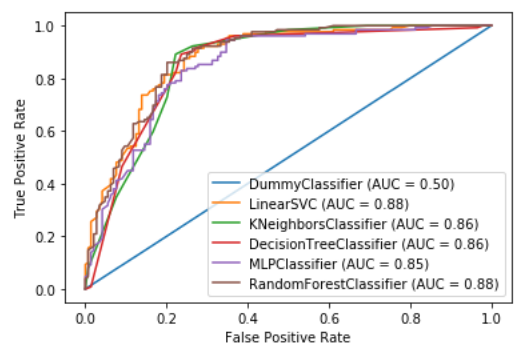
\includegraphics[width=150mm]{imagenes/ROC}}
\end{figure}

\section{Segmentación}

\end{document}
